\documentclass[12pt]{article}
\usepackage{amsmath,amssymb,amsthm}
\usepackage{graphicx}
\usepackage{subcaption}
\usepackage{float}
\PassOptionsToPackage{hyphens}{url}\usepackage{hyperref}\usepackage{color}
\usepackage{enumitem}
\usepackage{tabularx}
\usepackage[sorting=none]{biblatex}
\usepackage[raggedrightboxes]{ragged2e}
\setlength{\headheight}{15pt}
\usepackage{fancyhdr}

\usepackage{lineno}
\linenumbers

\usepackage[table,xcdraw]{xcolor}
\usepackage[normalem]{ulem}
\useunder{\uline}{\ul}{}


% figure and bibliography source
\addbibresource{../prime-editing.bib}
% add figure path
\graphicspath{ {../figures/} }
% reduce margin
\usepackage[margin=1in]{geometry}
% increase title font size
\usepackage{titling}
\pretitle{\begin{center}\Huge\bfseries}

\pagestyle{fancy}

\setlist[enumerate]{itemsep=0mm}

\title{PE Ensemble: An Interactive Review of In-silico Prime Editing Guide Design Tools}
% \author{Peiheng Lu}

\begin{document}
% no date
\date{}
\maketitle

\begin{abstract}
    Prime editing is a novel genome editing technology that enables precise base editing without the need for double-strand breaks. The design of prime editing guides is a critical step in the prime editing workflow. In this review, we evaluate the performance of several in-silico prime editing guide design tools. We compare the quality of the guide designed by these tools, and to improve the usage of these state of art tools, they were reimplemented and integrated into a single web base application. Additionally, we provided the ability to aggregate the results from multiple tools using ensemble learning to improve the overall guide design quality.
    Thus, with the on and off target activity of prime editing quantified, we can provide a complete overview of the outcome of using a specific pegRNA sequence on a specific target loci in a specific cell line. This should noticeably improve the safety and efficiency of prime editing, and thus accelerate its clinical application.
    Thus, with the on and off target activity of prime editing quantified, we can provide a complete overview of the outcome of using a specific pegRNA sequence on a specific target loci in a specific cell line. This should noticeably improve the safety and efficiency of prime editing, and thus accelerate its clinical application.

    \textbf{Keywords:} Prime editing, Machine Learning, in-silico tools, Ensemble Learning
\end{abstract}

\newpage

\section{Background}

Prime editing is a versatile and precise genome editing technology that enables the introduction of all 12 possible base-to-base conversions as well as insertions and deletions without the need for double-strand breaks\cite{liudavidr.SearchreplaceGenomeEditing2019}. 

The versatility of prime editors comes from the fusion of a reverse transcriptase (RT) and a Cas9 nickase (nCas9) to a prime editing guide RNA (pegRNA) (\autoref{fig:prime-editing}). After the guide RNA binds to the protospacer, the nCas9 creates a single-strand break in the complementary strand, which allows the RT to copy the edited sequence from the pegRNA into the target DNA. This mechanism enables theoretically any types of edits, as RT can be an arbitrary sequence of nucleotides\cite{liudavidr.SearchreplaceGenomeEditing2019}.  

\begin{figure}[ht]
    \centering
    \begin{subfigure}{0.5\textwidth}
        \includegraphics[width=\textwidth]{prime-editing-process.png}
        \caption{Prime editing mechanism}
        \label{fig:prime-editing}  
    \end{subfigure}
    \caption{(a) shows the mechanism of prime editing. The prime editing guide RNA (pegRNA) binds to the target DNA, and the nCas9 creates a single-strand break in the complementary strand. The reverse transcriptase (RT) then copies the edited sequence from the pegRNA into the target DNA.}
    \label{fig:figure-1}
\end{figure}

More than 6,000 disorders are known to be caused by various types of mutations in the genome, with around 300 new genetic disorders being discovered each year\cite{petraityteGenomeEditingMedicine2021}. Up to 90\% of these disorder-inducing mutations can be corrected using prime editing\cite{kantorCRISPRCas9DNABaseEditing2020}. However, its clinical application is significantly limited by its relative low editing efficiency at certain target loci.  Empirical methods could be used to identify prime editing guides with high editing efficiency, but they are time-consuming and expensive. Therefore, in-silico prediction tools have garnered significant interest in the scientific community.

\subsection*{In-silico Prime Editing Guide Design Tools}

A number of in silico on target prediction tools have been developed to predict the efficiency of prime editing guides. 

At the same time, deep learning approaches analysing the raw sequence data have also been developed.

DeepPE is one of the earliest in-silico prime editing guide design tools leveraging deep learning to predict the on-target activity of prime editing guides\cite{kimPredictingEfficiencyPrime2021}.

PRIDICT 2 makes a further step towards improving the prediction accuracy by updating the data preprocessing and model training step. By implementing multitask learning sharing the embedding and bidirectional RNN layers, PRIDICT 2 is able to predict the editing efficiency of prime editing guides with higher accuracy than its predecessor\cite{mathisMachineLearningPrediction2024}. 

This article provides a comprehensive review of the performance of these in-silico prime editing guide design tools, and makes them available through a unified interface, PE Ensemble.

\begin{figure}
    
\end{figure}
\section{Methods}

\subsection*{Data Acquisition and Preprocessing}

The dataset used in this study was obtained from the DeepPrime and PRIDICT studies\cite{mathisPredictingPrimeEditing2023,mathisMachineLearningPrediction2024,yuPredictionEfficienciesDiverse2023}, which contains around 220,000 and 110,000 prime editing guides-target pairs, respectively.

A set of functions were implemented to handle the conversion between formats required by different models. For datasets with fold information recorded, the corresponding trained models were preserved in the ensemble. While for datasets without fold information, a 5-fold cross-validation split used by DeepPrime and PRIDICT 2.0 was applied, and the models were retrained on the new folds.

A standardized format was devised 

Since the DeepPrime dataset does not contain a wide enough flank sequence of the target site for the PRIDICT model, padding was applied when converting the DeepPrime dataset to the PRIDICT format. 

\subsection*{Ensemble Learning}

Three ensemble learning approaches were investigated in this study: weighted average, bagging and AdaBoost. The algorithms were implemented in Python, but without the use of Scikit-learn ensemble library, as it does not support having different types of base learners in the ensemble.  


However, no significant difference in performance was observed among the three ensemble learning methods ($p>0.1$, paired t-test across corresponding folds, \autoref{appendix:ensemble}), possibly due to the high correlation in error between the base models (Add figure here). The weighted average method was chosen for the final implementation due to its simplicity and ease of interpretation.
\section{Results}

We present PE Ensemble, a web-based application that integrates multiple in-silico prime editing guide design tools. PE Ensemble provides a user-friendly interface for users to design prime editing guides and evaluate their on-target efficiencies. The application also allows users to aggregate the results from multiple tools using weighted mean ensemble learning to improve the overall guide design quality.
\input{../sections/discussion.tex}

\newpage
\appendix

\section{Appendix}

\subsection{Ensemble Learning Methods}
\label{appendix:ensemble}

Three ensemble models in total was investigated in this study: Weighted Average, Bagging and AdaBoost. 

As the name suggests, weighted average produces the final prediction by taking the weighted mean of the predictions from the base models, using the performance as measured by the Spearman correlation between the predicted and observed on-target activity as the weight. 

Bagging is a method that trains multiple models on different subsets of the training data, hoping to 

AdaBoost is a boosting ensemble method that trains multiple models sequentially. 

\begin{figure}[h]
    \centering
    \begin{subfigure}{0.4\textwidth}
        \centering
        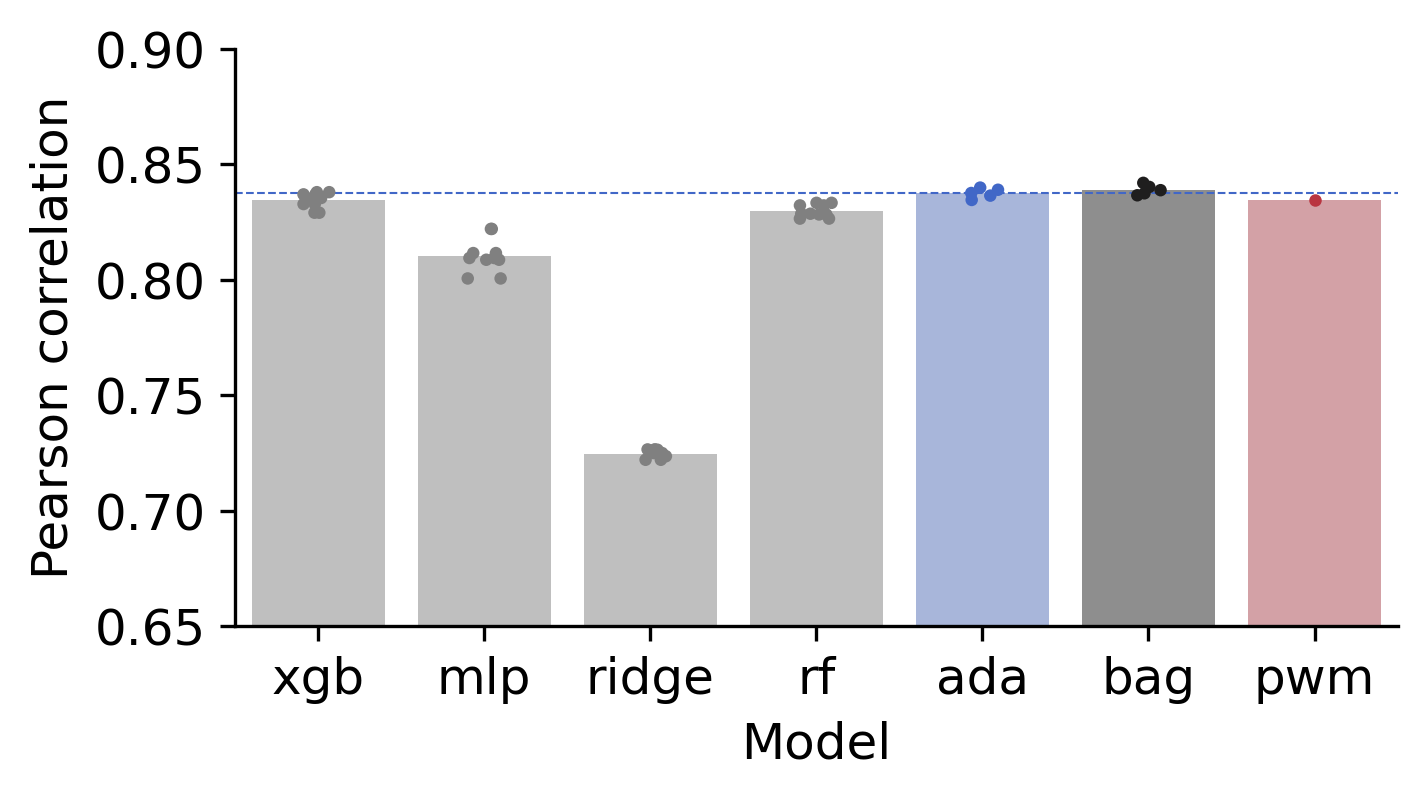
\includegraphics[width=\linewidth]{ensemble_comparison_Pearson.png}
        \caption{Pearson correlation}
    \end{subfigure}
    \begin{subfigure}{0.4\textwidth}
        \centering
        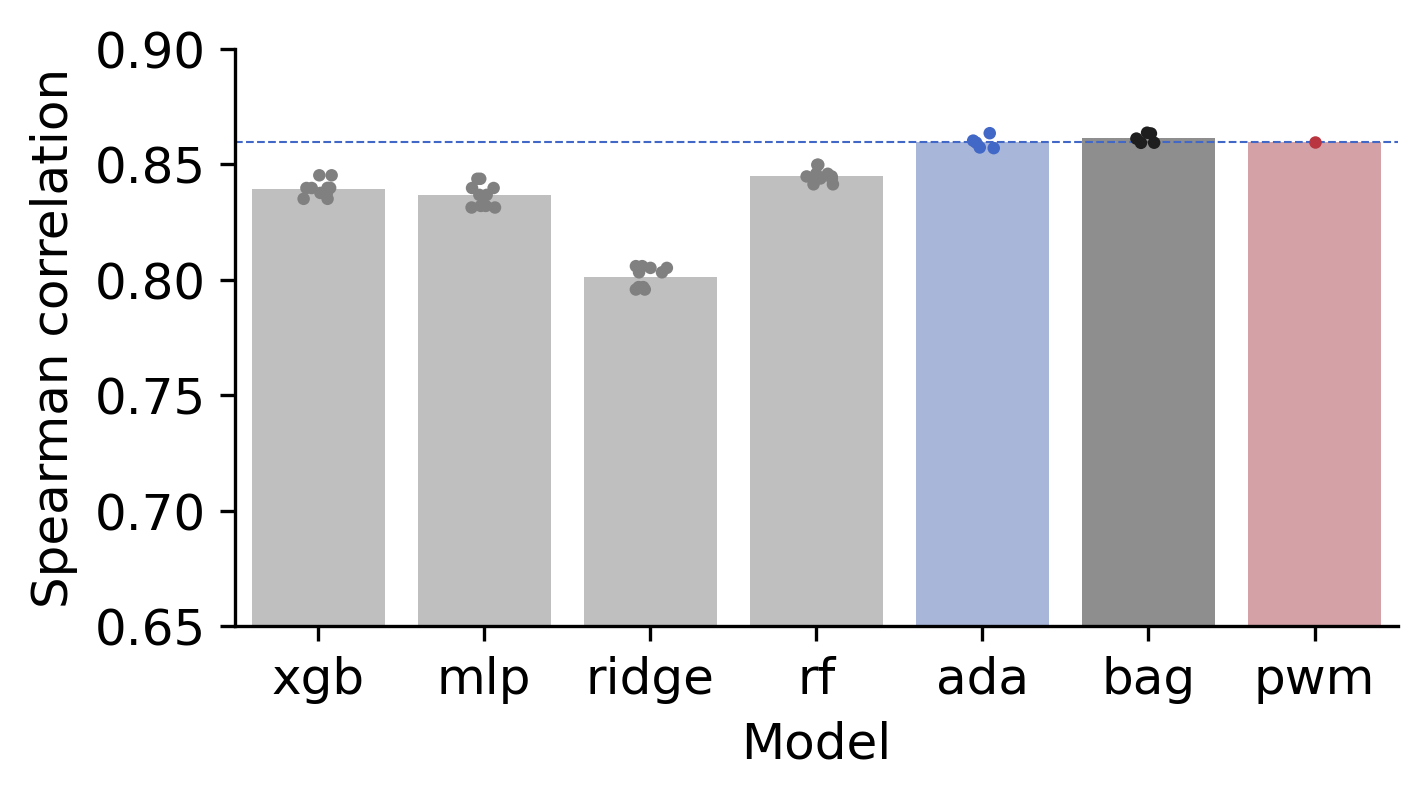
\includegraphics[width=\linewidth]{ensemble_comparison_Spearman.png}
        \caption{Spearman correlation}
    \end{subfigure}
    \caption{Comparison of ensemble learning methods' performance using (a) Pearson correlation and (b) Spearman correlation.}
    \label{fig:ensemble_comparison}
\end{figure}

\newpage
\printbibliography
\end{document}